\documentclass[10pt,b5paper,twoside,openany]{memoir}




%%% Packages 
\usepackage[utf8]{inputenc}
\usepackage[danish,english]{babel}
\usepackage{pdfpages}%include pdfs
\usepackage{amsmath}
\usepackage{amssymb}
\usepackage{float}
\usepackage{tikz}
\usepackage{blindtext}% dummy text
\usepackage{fancyhdr}
\usepackage{titlesec}
\usepackage[font={small}]{caption}
\usepackage{enumitem}
\usepackage[backend=biber,sorting=none]{biblatex}
\usepackage{csquotes}
\addbibresource{disbib.bib}

\DeclareUnicodeCharacter{0308}{.}

\usepackage{listings}
\usepackage{xcolor}
%% Colors 
\definecolor{codegray}{rgb}{0.5,0.5,0.5}
\definecolor{dtured}{rgb}{0.60, 0.00, 0.00}
\colorlet{thecolor}{dtured!100!}
\definecolor{thechptclr}{gray}{0.6}
\definecolor{thecaptionclr}{gray}{0.6}
\definecolor{gray20}{gray}{0.20}
\definecolor{gray40}{gray}{0.40}
 
\lstdefinestyle{mystyle}{
    keywordstyle=\color{magenta},
    numberstyle=\tiny\color{codegray},
    stringstyle=\color{codepurple},
    basicstyle=\ttfamily\footnotesize,
    breakatwhitespace=true,         
    breaklines=true,                 
    captionpos=b,
    keepspaces=true,                 
    numbers=left,                    
    numbersep=5pt,                  
    showspaces=false,                
    showstringspaces=false,
    showtabs=false,                  
    tabsize=2
}
 
\lstset{style=mystyle}

\pagenumbering{roman}

\title{The Title}

\author{First Last}
\date{22$^{th}$ October, 2022}

%%%%%%%%% WRITE THE SECTION NAME IN THE HEADER %%%%%
%\pagestyle{headings}

\chapterstyle{tandh}

% adjust caption formatting (memoir)
\captionnamefont{\bfseries} 
\captiondelim{. }
\changecaptionwidth
\captionwidth{5in}
\captionsetup{belowskip=0pt}


%%%%%%%%%% customization: formatting for Figure, Table, Equation references
\usepackage{graphicx}
%running fraction with slash - requires math mode.
\newcommand*\rfrac[2]{{}^{#1}\!/_{#2}}
\newcommand{\fig}[2]{\textbf{Figure~\ref{#1}{#2}}} 
\newcommand{\tab}[2]{\textbf{Table~\ref{#1}{#2}}} 
\newcommand{\tabb}{\hspace*{2em}}
\newcommand{\sub}[1]{\mbox{(\textbf{#1})}} % formatting for subfigure label within a caption
\newcommand{\prog}[1]{\texttt{#1}}

\newcommand{\fixme}[1]{\textbf{\underline{#1}}} 
%%%Font size on chapters, sections and subsections
\newcommand*{\justifyheading}{\raggedleft}

\titleformat*{\section}{\LARGE\bfseries}
\titleformat*{\subsection}{\Large\bfseries}
\titleformat*{\subsubsection}{\large\bfseries}
\titleformat*{\paragraph}{\large\bfseries}
\titleformat*{\subparagraph}{\large\bfseries}



%###########################
\begin{document}
%###########################
\setcounter{page}{0}
% Source: https://www.overleaf.com/learn/latex/How_to_Write_a_Thesis_in_LaTeX_(Part_5)%3A_Customising_Your_Title_Page_and_Abstract

% \begin{titlepage}
\begin{center}
    \vspace*{1cm}
        
    \Huge
    \textbf{Thesis Title}
        
    \vspace{0.5cm}
    \LARGE
    Thesis Subtitle
        
    \vspace{1.5cm}
        
    \textbf{Author Name}
        
    \vfill
        
    A thesis presented for the degree of\\
    Doctor of Philosophy
        
    \vspace{0.8cm}
        
    % \includegraphics[width=0.4\textwidth]{logo}
        
    \Large
    Department Name\\
    University Name\\
    Country\\
    Date
        
\end{center}
% \end{titlepage}

\frontmatter

\noindent
\textbf{Preface}\\
The work in this thesis was carried out between month year and month year in fulfillment of the requirements for acquiring a PhD degree. 
The work was mainly carried out at the Novo Nordisk Foundation Center for Protein Research under the Faculty of Health and Medical Sciences at the University of Copenhagen.
The work was conducted under the supervision of Associate Professor Simon Rasmussen and Professor Søren Johannes Sørensen. In addition, part of this work was carried out during a four-month external stay at ... .
The funding for this PhD comes from the Novo Nordisk Foundation (grant no: NNFX). \\

\noindent
Copenhagen, September 2022\\
\noindent
Joachim Johansen
\noindent
\textbf{Author}\\
\noindent Joachim Johansen, MSc. cand. polyt.\\
\textit{Novo Nordisk Foundation Center for Protein Research, Faculty of Health and Medical Sciences, University of Copenhagen}\\
\newline
\newline

\noindent \textbf{Academic Supervisors}\\
Associate Professor Simon Rasmussen, \textbf{Principal supervisor}\\
\textit{Novo Nordisk Foundation Center for Protein Research, Faculty of Health and Medical Sciences, University of Copenhagen}
\newline
\newline
Professor Søren Johannes Sørensen, \textbf{Primary co-supervisor}\\
\textit{Section of Microbiology, Department of Biology, University of Copenhagen, Copenhagen, Denmark}

\noindent \newline  \newline \textbf{Assessment Committee}\\
Associate Professor Nicholas M I Taylor\\
\textit{Novo Nordisk Foundation Center for Protein Research, Faculty of Health and Medical Sciences, University of Copenhagen}
\newline
\newline
Professor Mads Albertsen\\
\textit{Center for Microbial Communities, Aalborg University, Denmark}
\newline
\newline
Dr Eduardo Rocha\\
\textit{Microbial Evolutionary Genomics, Institut Pasteur, France}
\chapter{Acknowledgements}
Three years of computational science that worked out well has been condensed into this dissertation. For all the time that was not smooth sailing, I have been very lucky to have the support of many that I wish to acknowledge. First, a big thanks to Simon Rasmussen for all your support, energy and boundless enthusiasm for computational sciences and bioinformatics. Thanks to Søren Sørensen for co-supervision and for sharing your insights on microbiology. I would like to acknowledge all of my colleagues in the Rasmussen Lab who spent the entire or a great part of the time with me during this PhD. To the PhD-students of the group (Henry, Rosa, Marie Louise, Ricardo, Roman, Leonardo, Pau, Kirstine and Arnor) and postdocs (Jakob, Jonas, Lili, Katrine and Knud). Thanks for the many trips to the coffee machine, excessive cake meetings and amazing scientific retreat in Malta. Thanks to the CPR administration for supporting our scientific endeavors and to the SPA members for making all the hours at CPR more enjoyable with great events, beers and hygge.\\
I would also like to thank my collaborators and friends overseas. Thanks to Damian Plichta for many years of academic mentoring and collaboration, which started with running bash commands at Clinical Microbiomics and now a finished dissertation. Thanks to Hera Vlamakis who inspired me to take the final step and embark on the PhD. In addition, I am grateful to Ramnik J. Xavier for both his supervision and on-site and remote academic hosting during this PhD. Thanks to Thomas Pedersen and Eric Brown for sunny lunches and coffee breaks during my Autumn in Boston and also, by the way, doing three years of incredible lab work to verify my computational master thesis project and publish it. Furthermore, I wish to thank Kenya Honda and Koji Atarashi for their collaboration and inspiring work on human longevity and the microbiome. To my abroad-family in the US, Damian and Jesper, thanks for great hostmanship, superb company and slow mornings with several shots of espresso and long discussions on economy and technology.\\
Thanks to Christina for supporting me throughout all the ups and downs and painstakingly reading, editing, checking and \textit{regulating} this dissertation. Finally, thanks to my family and friends for your unconditional support during this journey.


%%%%% Table of Content
%\cleardoublepage
\renewcommand*\contentsname{Table of contents}
\tableofcontents*

%% Font stuff 
\chapter{English summary}

The human gut microbiome harbors several groups of residents including the bacterial, archeal, eukaryotic and viral kingdom. The bacterial kingdom is the most well studied and acknowledged for its significant role in metabolic processes and immune development important to the human host. The bacterial community is also a big contributor to the genetic pool and biomass of the gut which underscores its functional significance in the ecosystem. Yet, bacterial infecting viruses, known as bacteriophages, are suggested to equal or outnumber bacteria in the human gut. Due to the predatory mode of bacteriophages, they may exert a profound regulative role on bacterial constituents during health and disease.

\noindent
In this thesis I explore computational frameworks using established methods from Artificial Intelligence and bioinformatics to mine and discover novel biological diversity including bacteria and viruses from human gut microbiomes. In the \textbf{first} article we present VAMB, a new method for binning. VAMB uses variational autoencoders to represent metagenomic sequences before the representation is clustered using a novel algorithm. We apply this method to a collection of synthetic metagenomes and thus demonstrate that Vamb creates more accurate bins than comparable software. By binning a large natural dataset with 1,000 human feces samples and almost 6 million assembled sequences, we demonstrate that Vamb can recreate bacterial strains with high phylogenetic resolution. In the \textbf{second} article we showcase how VAMB can be utilized for viral metagenomic binning in a framework we named PHAMB. Virus genomes present a different binning challenge compared to bacterial genomes as they are composed of smaller and more fragmented sequences in \textit{de novo} assemblies. Even though VAMB was not originally designed with viruses in mind, our analysis shows that it successfully bins both bacteria and virus genomes in parallel, which facilitates downstream community analysis in metagenomic datasets. Importantly, we found that binning improves the total recovery and quality of virus genomes compared to single-sequence virus recovery across three different datasets. In the \textbf{third} article we apply viral genome binning to delineate viral populations in centenarian gut microbiomes to reveal novel viral diversity that may promote human longevity. Healthy aging seems to promote a rich and diverse virome that interacts with beneficial dominant bacterial hubs in the microbiome. As bacteriophages represent a dynamic component of the microbiome, they may provide health promoting functional capabilities to the gut bacteria they infect. In support of this hypothesis, we discovered that centenarian bacteriophages encode key enzymes found in bacterial metabolic systems related to the conversion of sulfate to sulfide and methionine to homocysteine. Together with its bacterial part, the centenarian gut microbiome displayed increased potential for the conversion of sulfate to sulfide. A greater metabolic output of microbial hydrogen sulfide may in turn support mucosal integrity and resistance to pathobionts.

\noindent
This thesis presents methodological frameworks for organizing bacteria and viruses in the human gut microbiome into biological meaningful entities and dissecting their potential impact on the human host. Until future generation sequencing technologies become cost effective, accurate and gradually replace current methods for studying metagenomics, computational methods such as metagenomics binning will be necessary for discovering and delineating bacterial and viral diversity and their intricate dynamics.
\chapter{Dansk resumé}

Det menneskelige tarmmikrobiom er vært for adskillige grupper af mikroorganismer, herunder bakterier, arkæer, eukaryoter og virus. Tarmbakterier er den mest undersøgte af disse og er anerkendt for dets rolle i tarmmetabolismen og immunsystemets udvikling, begge af stor betydning for den menneskelige vært. Desuden udgør bakterier en stor del af den genetiske arvemasse i tarmen som understreger deres funktionelle betydning i økosystemet. En mindre undersøgt gruppe i tarmens økosystem er bakterieinficerende virus, også kendt som bakteriofager. Bakteriofager er anslået til at udligne eller overstige antallet af bakterier i tarmen. Givet deres destruktive interaktion med bakterier, kan de have en stor betydning for bakteriebalancen under raske og sygdomsbetingede tilstande. 
I denne afhandling udforsker vi algoritmer og computerbaserede metoder med etablerede metoder fra kunstig intelligens og maskinlæring til at opdage og karakterisere tarmens biodiversitet, herunder bakterier og vira fra menneskelige tarmmikrobiomer. I den \textbf{første} artikel præsenterer vi VAMB, en computerbaseret algoritme til metagenomisk binning, hvilket kan oversættes til gruppering. VAMB er baseret på en variational autoencoder til at repræsentere metagenomiske sekvenser som nemmere kan splittes og grupperes til samlede bakterielle genomer. I artiklen har vi demonstreret at VAMB er bedre end tilsvarende værktøjer til at gruppere syntetiske metagenomer og genskabe bakteriestammer. Ligeledes har vi anvendt VAMB på et stort metagenomisk datasæt baseret på 1000 humane fæces prøver med næsten 6 millioner sekvenser og vist at VAMB kan genskabe bakteriestammer med høj fylogenetisk præcision. I den \textbf{anden} artikel beskriver vi, hvordan VAMB kan bruges til gruppering af tarmens virus genomer i en metode vi har kaldt PHAMB. Binning af virus genomer er betinget af andre udfordringer end bakterielle genomer, da deres genomer typisk er mindre og mere fragmenterede. Selvom VAMB ikke oprindeligt blev designet specifikt for virus, har vi vist at det kan anvendes til at genskabe både bakterielle og virale genomer parallelt, hvilket muliggør undersøgelse af begge biologiske domæner i metagenomiske datasæt. Desuden etablerer vi at at binning forbedrer den totale rekonstruktion og kvalitet af virusgenomer på tværs af tre forskellige datasæt. I den \textbf{tredje} artikel anvender vi begge metoder (VAMB og PHAMB) til at karakterisere og undersøge bakterielle og virale populationer i tarmmikrobiomer fra hundredårige samt yngre kontrolgrupper. I studiet opdager vi først og fremmest ny viral diversitet der potentielt kan fremme menneskets levetid. Desuden, observerer vi at hundredåriges tarmmikrobiom huser et rigt og mangfoldigt virus system der interagerer med gavnlige bakterielle populationer. Det siges at bakteriofager kan bidrage med ekstra funktionel arvemasse til bakterierne de inficerer. Vi opdagede i forlængelse af denne hypotese at bakteriofager integreret i bakterier fra hundredårige bidrager med enzymer der faciliterer vigtige trin i bakterielle metaboliske systemer relateret til omdannelsen af sulfat til sulfid og methionin til homocystein. Tilsammen viste vi at hundredåriges tarmmikrobiom har et øget metabolisk potentiale for omdannelse af sulfat til sulfid, hvilket kan have stor betydning, da en øget mængde af svovlbrinte i tarmen kan understøtte tarmens integritet og resistens over for patogener.
Afhandlingen beskriver computerbaserede metoder til at organisere bakterier og virus arter i det menneskelige tarmmikrobiom og en dissektion af deres potentielle indvirkning på den menneskelige vært. Indtil fremtidige sekventeringsteknologier bliver omkostningseffektive, nøjagtige og gradvist erstatter nuværende sekventeringsmetoder til at studere metagenomiske prøver, vil værktøjer baseret på binning være nødvendige for at etablere bakteriel og viral diversitet samt forstå deres indviklede dynamik.

%\cleardoublepage
\chapter{List of publications}
This thesis is based on the following three manuscripts: 

\begin{enumerate}[label=PAPER \Roman*.]


\item \textbf{Johansen, J}; Plichta R.D.; Nissen, J.; Jespersen L. M; Shah A., S.; Deng, L.; Stokholm, J.; Bisgaard, H., Nielsen S.; D., Sørensen J; S., Rasmussen, S.† (2022). \textit{Genome binning of viral entities from bulk metagenomics data}. Nature Communications, Article 965.
\newline
In review, Nature Microbiology
\end{enumerate}

\noindent
I have contributed to the following articles during my PhD, which are not included in this thesis:
\begin{enumerate}[label=PAPER \Roman*.]

\item Jespersen L. M; Munk, P.; \textbf{Johansen, J}; Kaas, R.; Webel, H.; Vigre, H.; Nielsen B., H; Rasmussen, S.; Aaastrup, F.† (2022)
\textit{Global within-species phylogenetics of sewage microbes suggest that local adaptation shapes geographical bacterial clustering}
\newline

\item Schubert, L; Hendriks, Ivo. A; Hertz, E; Wu, Wei; Sellés-Baige, S; Hoffmann, S; Viswalingam, K.S; Gallina, I; Pentakota, S; Benedict, B; \textbf{Johansen, J}; Apelt, K; Luijsterburg, M; Rasmussen, S; Lisby, M; Liu, Y; Nielsen, M.L; Mailand, N and Duxin P.J† (2022) \textit{SCAI promotes error-free repair of DNA interstrand crosslinks via the Fanconi anemia pathway}
EMBO reports. https://doi.org/10.15252/embr.202153639

\end{enumerate}

\noindent
† Corresponding author 
\chapter{Thesis content and overview}\label{overview}
The central theme of this Ph.D. has been the development and application of methods to delineate bacterial and viral diversity from metagenomics. Successful organization of bacteria and viruses into ecological species hubs allows analysis of their interactions and the implications on the metazoan host like humans. The majority of microbiome studies that explored human gut biodiversity and its implications on human health have focused primarily on the bacterial constituents. The reason for this was twofold: (1) the virome (the collective of viruses in the environment) was mostly explored in viral-enriched metagenomic samples with \textit{in vitro} isolated viral fractions and (2) the feasibility of exploring the virome from samples without viral preprocessing was barely described and problematic due to bacterial contamination. However, the growing wave of bulk/non-enriched metagenomic samples collected from the human gut, soil and marine environments is continuing to dwarf the number of collected viral-enriched metagenomic samples, which corresponds to metaviromes. Thus, there is a profound need for standardized methods to extract and explore the virome from bulk metagenomics due to their influence in the environment.

\medskip
\noindent
In \textbf{Chapter 1}, I provide a brief history on the discovery of bacterial and viral diversity in metagenomics and its current state and challenges. In addition, I outline a concise review on virus biology and dynamics with bacteria and altogether the possible implications to metazoan hosts like humans. In \textbf{Chapter 2}, I describe the bioinformatic methods and concepts with a focus on genome binning, genome annotation, machine learning and genome-driven ways to connect bacteria and viruses. In \textbf{Chapter 3}, I list and expand on the research objectives pursued during this Ph.D project. In \textbf{Chapter 4}, I describe the three major studies included in this thesis related to metagenomics binning of bacteria and viruses, and a study on the gut virome in humans with extreme longevity. In \textbf{Chapter 5}, I summarize and discuss the major results of the three studies included. In \textbf{Chapter 6}, I discuss future perspectives and suggestions for improved bacterial and virome analysis in metagenomics. \textbf{Chapter 7} contains ethical and legal permits and approvals required for the clinical and animal studies. \textbf{Chapter 8} includes the manuscripts included in this dissertation.

\clearpage



%%%%%%% PREFACE CHAPTERS INCLUDE%%%%%%%%%%%%%%%%%%%%%%%%%%%%%%

\mainmatter
\setcounter{page}{1}

%%%%Put number on subsubsection:
\setcounter{secnumdepth}{3}
\newpage

%%%%%%%%%%% INTRODUCTIOn %%%%%%%%%%%%%%%


%\titlespacing\section{0pt}{0pt}{\parskip}{-\parskip}

%% Header
\makepagestyle{dtu}

\makeoddhead{dtu}{\leftmark}{}{\thepage}
\makeevenhead{dtu}{\thepage}{}{\leftmark}

\makeheadrule{dtu}{\textwidth}{0.3pt}
\pagestyle{dtu}
\aliaspagestyle{chapter}{dtu}

\cleardoublepage
\begingroup

\chapter{Background}
\section{The study of human gut biodiversity through DNA}

Modern DNA sequencing technology has provided a way to read into the building blocks of life, from the first cultured bacteria to the first human genome \cite{Koonin1996-vp,Lander2001-vu}. Today, we only need a biological specimen with DNA to sequence and read the genetic blueprint to determine who is there. Before modern sequencing technology brought us this far, we had to differentiate between bacteria by looking at them under a microscope based on their morphology, thanks to the inventions of Van Leeuwenhoek \cite{Lane2015-yo}. Culturing techniques have further improved this method by allowing single-culture isolates. However, In a mixed biological sample from soil, ocean water or feces that contains thousands of different bacterial species, isolating, culturing and determining every single one is an impossible task \cite{Staley1985-zr}. As not all bacteria are obligate aerobic bacteria, but obligate anaerobes like the trillions of bacteria in the human gut, many would not survive culturing on a petri dish.\\

\noindent
A more precise determination of \textit{who} a bacteria is can be made through its genetic blueprint of the 16S ribosomal RNA gene \cite{Nr1985-yh}, which is an excellent phylogenetic marker for placing bacteria and archaea in the tree of life. The 16S rRNA gene is highly conserved between different bacteria and archaea due to its species specific signature of the letters A, T, C and G, which makes it useful for bacterial identification. Therefore, 16S rRNA sequencing technology has been an incredible tool for studying who is present in metagenomic samples from the human gut and allowed the first characterisations of commensal bacteria in the gut microbiome of hundreds of people. However, the metabolic and phenotypic traits of bacteria in an environment goes beyond the 16S rRNA marker gene. As a result, the desire to study the full genetic repertoire and \textit{what} bacteria can do within an environment lead to the advent of modern shotgun sequencing.

\section{Resolving uncultivated genomes in metagenomics}

Shotgun sequencing ushered in an era of genome-resolved metagenomics leading to the recovery of genes from novel uncultivated organisms \cite{Venter2004-ce}. Simultaneously, the popularity of metagenomics exploded as it became abundantly clear that the human microbiome is strongly correlated with health and markedly changed in disease states \cite{Lloyd-Price2016-qf}. High-throughput Illumina shotgun sequencing produces only short random fragments of DNA but in vast quantities. Powerful genome assembly algorithms were designed to utilize small repetitive sequence fragments to identify sequence overlaps and establish long continuous sequences, which were coined contigs. The strategies to resolve multiple uncultivated genomes from a random “soup” of contigs included (1) basic sequence alignment to a database of cultured sequence isolates (2) contig-binning based on similar GC-frequencies (3) tetranucleotide frequencies and (4) differential read-coverage. The read-coverage strategy (4) was based on the idea that contigs from the same genome should display a roughly similar sequencing depth. This data-driven strategy represented a powerful concept that many modern binners were later designed to leverage for binning genes or contigs into metagenomic assembled genomes (MAGs)\cite{Albertsen2013-en,Nielsen2014-vu,Kang2019-su}. The initial strategy used to determine when a MAG corresponded to a complete genome was based on the presence of essential bacterial single-copy genes (bacterial markers) \cite{Albertsen2013-en}, which is an approach still used to some extent today by bioinformatic tools like CheckM \cite{Parks2015-cs}.\\

\noindent
The presence of universal markers like the 16S rRNA gene and other single-copy gene markers in bacteria has enabled their identification in metagenomics and fuelled an explosion of known bacterial diversity during the last decades. Thus, the availability of bacterial genomic blueprints in the form of uncultivated bacterial genomes tallies hundreds of thousands across the human microbiome(s), ocean and soil \cite{Almeida2019-fk}. Meanwhile, the progress of developing databases containing genomes of other biotic constituents like fungi or viruses has been quite different. The reason why viruses were late to the party is due to several technical assembly challenges that will be addressed later, but most importantly they do not contain a universal virus marker gene. For the majority of people, viruses are considered obligate pathogens as we associate them to many types of diseases afflicted by human-infecting viruses, such as the Influenza virus. These types of viruses have represented the bulk of virus blueprints in databases for many years while the focus has been fixed on bacteria (Figure 1). As a result, most metagenomic sequences corresponding to an actual virus have resembled those in the current virus databases. From 2016 to 2018 (Figure \ref{fig:virushistory}) the number of uncultivated virus genomes exploded in the databases with 750,000 genomes when genomes mined from the first two large virus studies from ocean and soil were released \cite{Roux2016-yu,Paez-Espino2016-bb}. The success of these expansive viral studies could be attributed to the maturation of \textit{in vitro} protocols for concentrating viral particles, which enabled a greater space for viral assembly and identification.

\begin{figure}[H]
  \includegraphics[scale=1, width=1\textwidth]{pictures/mroux2019.pdf}
  \caption[VirusTimeline]{The figure illustrates a recent timeline going back to 2004 and the cumulative number of virus genomes uploaded to genome databases since then, including uncultured virus genomes (UViGs). In addition, major events related to virus discovery are notated across the timeline. Virus genomes cultured \textit{in vitro} from isolates are depicted as blue and green, where the green corresponds to reference genomes at ncbi (\url{https://www.ncbi.nlm.nih.gov/nuccore}). The discovery of uncultured virus genomes (yellow) began in early 2006 and has since then exceeded the number of reference genomes many times over. Figure modified from \textit{Minimum Information about an Uncultivated Virus Genome} \cite{Roux2019-dc}.
  }
  \label{fig:virushistory}
\end{figure}

\noindent
We now recognise that virus particles can be identified almost anywhere where they sometimes massively outnumber other cells like bacteria \cite{Breitbart2018-sj}. To most people, it might be surprising that there are trillions of viral particles around us without the capacity to infect us as they prey on other microscopic organisms like bacteria. The group of viruses preying on bacteria are known as bacteriophages (phages for short). We are now recognising their impact and presence as early studies have unraveled a dynamic and changing virus community during disease like inflammatory bowel disease \cite{Norman2015-eb,Clooney2019-nn}. Therefore, the search for potential viral culprits has begun in addition to beneficial bacteriophages with protective properties. In order to understand how bacteriophages could be implicated in disease as they do not infect humans, we have to consider the way phages interact with bacteria who directly influence the human immune system and metabolism.
\endgroup

\begingroup
\chapter{Methods} 
\section{Machine learning}

Machine learning (ML) is a subgroup of artificial intelligence (AI), which encompasses a long range of computational models that learns from high quantities of data to classify and recognise patterns. The learning is either directed in a \textit{supervised} way with labeled data structures or in an \textit{unsupervised} way where the system aims to identify patterns without a predefined structure or truth. In both cases (supervised or unsupervised) the model is working to minimize a loss or cost function that captures the deviation of the predicted or generated output relative to the ground truth or input.\\

\noindent
Within the realm of microbiome research, ML models have been applied in several cases for the purpose of classification. ML have been developed for host phenotyping using the microbiome composition and bacterial species abundance as the only information and can successfully stratify patients based on their microbial signature \cite{Pasolli2016-pi,Statnikov2013-gz}. Some ML models also include functions for assessing feature importance on model performance, which have been used to identify discriminative bacterial strains that exacerbate a disease phenotype \cite{Pasolli2016-pi}. The features represent measurable or categorical units in the dataset, such as the abundance of bacterial species or whether the sample is from a control or case patient. Microbial features can be combined with other omics such as metabolomics, gene-expression or host clinical data to increase the models ability to differentiate phenotypes \cite{Zhou2019-nc}. The choice of ML method to use for each application largely depends on the data, method preference and importantly whether or not the data is complete with truth-labels to facilitate supervised learning of the model. Methods that have been used for supervised learning in microbiome studies are manyfold and include logistic regression, Linear Discriminant Analysis, support vector machines (SVMs), naive bayes classifiers and artificial neural networks \cite{Marcos-Zambrano2021-eg}. For one of the publications in this dissertation, we leveraged the Random Forest (RF) model.

\subsection{Random Forest}

The RF model is an ensemble of multiple decision trees in which the performance is evaluated based on pre-labelled data. Each individual tree in the RF makes a class prediction and the majority vote across all trees becomes the final prediction, thereby employing the “wisdom of the crowds” instead of relying on a single classifier. For a given training dataset with x number of observations characterized by y variables, the RF model constructs a prespecificied number of random decision trees (Figure \ref{fig:RF}). The randomness comes into play as the y-variables used to describe each observation are randomly sampled at each node in the decision trees.

\begin{figure}[H]
  \begin{center}
    \includegraphics[scale=1, width=1\textwidth]{pictures/Random_forest.png}
  \end{center}
  \caption[VirusTimeline]{The Random Forest (RF) contains a predefined number of decision trees, which are randomly constructed resulting in n independent decision trees. A trained RF model works by receiving an input that is processed by each decision tree in the forest, which produces an independent prediction of the class based on the input. The final prediction is based on a majority vote across all trees to produce a final prediction.
  }
  \label{fig:RF}
\end{figure}

\noindent
The RF model is evaluated using a method called bagging as it randomly samples with replacements from the observations in the dataset. This also means that some observations are not sampled and therefore “bagged” in the out of bag (OOB) set, which can be used to test the accuracy of the final tree ensemble. Based on the OOB observations, an OOB-error is derived and provides an immediate estimate of the RF model's accuracy. When training other supervised ML methods like linear regression classifiers or SVMs that do not employ OOB, \textit{k}-fold cross validation (CV) is an ideal approach for testing the accuracy of the model during training and ensuring that the accuracy is calculated based on observations not used in estimating the parameters of the model. With CV, the observations are split into \textit{k} number of partitions; then the training is performed \textit{k} times using one partition of the observations as the test dataset and the rest as training data. To achieve a final estimate on whether the ML model generalizes to new observations, the most important estimate of accuracy should ideally be calculated based on an independent dataset. An overfitted model may produce good results on the training data set but underperform on real-world data points.

\subsection{Variational autoencoders}

One of the artificial neural network methods that has received increased attention is the autoencoder that has proven useful for capturing structures in high dimensional data with many features per observation such as single-cell RNA-seq and multi-omics data \cite{Ma2019-mp,Wang2021-ne}. Autoencoders are designed to receive an input and encode it into a compressed representation coined the latent representation, which can be decoded to reconstruct the input. The autoencoder is trained to minimize the difference between the original input and decoded output by minimizing a loss function that captures this difference numerically (Figure \ref{fig:encodedecode}).

\begin{figure}
  \begin{center}
    \includegraphics[scale=1, width=1\textwidth]{pictures/ML_autoencoder_schema.jpeg}
  \end{center}
  \caption[VirusTimeline]{A classic example of Autoencoders is the usage for reconstructing images. In the example depicted, the original input (image of a “2”) is encoded into a compressed representation and decoded into an output very similar to the original image. Illustration from: https://blog.keras.io/building-autoencoders-in-keras.html
  }
  \label{fig:encodedecode}
\end{figure}

\noindent
Autoencoders consist of a chain of artificial neural network (ANN) layers with a distinct architecture in which the first layer (that receives an input) has the same dimension of the last layer (which recreates the input). In the process of encoding a high-dimensional input $y$ into a low-dimensional compressed representation $z$, which can be decoded into an approximation of the original input $\hat{y}$ (Figure \ref{fig:VAE}), the network can capture important nonlinear structures in a dataset. The property for turning high-dimensional data into a low dimensional compressed representation $z$ makes the autoencoder a dimensionality reduction method as it learns to store all the relevant information in a few explanatory variables. An issue with the traditional autoencoder architecture is the fixation on encoding and decoding an input with as little loss of information as possible, which can lead to overfitting. If the autoencoder is overfitted, the encoder may map any data point to an arbitrarily small segment of the latent space $z$ as real numbers where the decoder can still recreate the input but the position in latent space is structurally meaningless. The autoencoders’ mapping of an input $y$ into the latent space $z$ can therefore become completely arbitrary. This would effectively make the autoencoder produce gibberish when exposed to new data points. In addition, arbitrary mapping of input into latent space makes it impossible to cluster the latent representation $z$ into anything meaningful if unrelated data points are positioned close in latent space.\\
\noindent
With Variational autoencoders (VAE), the training is performed using a regularization technique to avoid overfitting and enforce structure to the data points in latent space. The key is to ensure that data points that are close in the input space are also close in the latent space, which makes clustering of the latent space more feasible. To achieve this, the input $y$ is encoded as a Gaussian $\mathcal{N}(\mu, \sigma)$ distribution with a mean $\mu$ and standard deviation $\sigma$ by a function $E(y)$ \ref{fig:VAE}), instead of a low-dimensional data point. From the latent distribution $p(z)$, a latent representation $z$ is sampled and decoded into $\hat{y}$, which makes the VAE a generative model. 

\begin{figure}[H]
  \begin{center}
    \includegraphics[scale=1, width=1\textwidth]{pictures/VAE.png}
  \end{center}
  \caption[VirusTimeline]{The Autoencoder and Variational Autoencoder (VAE) may have similar architectures as they both contain an input layer $y$ and output $\hat{y}$ layer with same dimensions, an encoder and decoder layer and a latent representation (center layer). However, the VAE encodes the input into a latent distribution $p(z)$ function that can be sampled from to reconstruct the input. Both methods can produce a latent representation $z$ for a group of high-dimensional data points that is more suitable for clustering and can be visualized in a lower dimensional space.
  }
  \label{fig:VAE}
\end{figure}

\noindent
For training the VAE, the loss function is composed of two terms \cite{Doersch2016-bo}; (1) a reconstruction error that represents the difference between the original input $y$ and the decoded output $\hat{y}$ and (2) a regularization term on the latent layer that enforces the encoder to return a gaussian distribution $\mathcal{N}$. The regularization term is expressed as the Kulback-Leibler (KL) divergence function that captures how well the encoded Gaussian distribution approximates a standard Gaussian distribution $\mathcal{N}(0,1)$ where $\mu$ is 0 and $\sigma$ is equal to 1. These two terms together make up The Evidence Lower BOund (ELBO) function also described as the variational lower bound. The ELBO can either be represented as the expected negative log likelihood plus the KL divergence, where the ELBO loss function is minimized during training of the VAE.

\begin{equation}
ELBO(y) = -\mathbb{E}_{E}[log(p(y|z))] - D_{KL}(E(y) \Vert p(z))
\end{equation}

\noindent
Or as an expression where the ELBO is maximized by minimizing the KL divergence while maximizing the expected log-likelihood.

\begin{equation}
ELBO(y) = \mathbb{E}_{E}[log(p(y|z))] - D_{KL}(E(y) \Vert p(z))
\end{equation}

\noindent
Ultimately, what we want to achieve using a VAE is to map similar values closely in the latent space. Compared to an ordinary autoencoder trained to decode arbritary data points into near exact recreations of the input, in the VAE the decoder samples from encoded Gaussian distributions of the input, which results in similar recreations of the input instead of near exact. The VAE’s capacity for encoding high-dimensional observations into meaningful low-dimensional numeric vectors without any prior labeling of observations makes it an unsupervised and powerful method for dimensionality reduction and clustering. Biological samples from patients or natural environments are characterized today with thousands of features produced by multi-omics, thus the VAE is getting more recognised as an appropriate tool for differentiating anything from cell types to human pathologies.  

\endgroup

%%% Introduction of each Project 
\begingroup
\chapter{Research objectives}
In \textbf{Chapter 1}, I have provided a brief and non-exhaustive overview on how bacteria and viruses are studied in metagenomics. In addition, I have provided a basis for understanding why the interaction of bacteria and viruses can be profound to an environment like the human gut microbiome. Current and future metagenomic studies like the “Million Microbiome of Humans Project”\footnote{news.ki.se/first-project-to-create-atlas-of-human-microbiome} do not provide metaviromes as it would double the sequencing efforts and the costs. The development of methods for extracting the virome from bulk metagenomes are important and represent a desired approach to facilitate virome analysis in future metagenomic studies. We set out to develop and explore methods to face the lack of metaviromes and enable investigations into ecological hubs of viruses and bacteria in microbiomes. Based on ongoing work related to metagenomic binners, we chose binning as our starting point and have worked toward generating both bacterial and virus genomes from bulk metagenomics with this technique.\\

\noindent
To pursue a framework for discovery of viral diversity in bulk metagenomics, I defined the following challenges:
\begin{enumerate}
    \item Establish or adapt a method to bin virus genomes in parallel with bacteria and estimate the success of virus recovery relative to metaviromes.
    \item Benchmark the framework from (i) for large scale discovery of viruses and bacteria in metagenomics, define how much viral diversity is captured and what diversity is missed.
    \item Investigate and re-analyse gut viromes in cohorts without metaviromics to expand our understanding of viral and bacterial hubs in different cases of health and disease. 
\end{enumerate}

\noindent
To expand on \textbf{Objective 1}, we planned to leverage paired metagenomics and metaviromics to evaluate and tune viral genome recovery in bulk metagenomic samples. We proposed to use the generative VAE model for phage binning, which was an ongoing project in the group. For developing and training the phage specific binning algorithm we used paired human gut microbiome and metavirome datasets from the COPSAC and Diabimmune (T1D) cohorts, where COPSAC is by far the largest paired metagenomic and metaviromic dataset produced as of this date. Using paired bulk metagenomic and metavirome data is crucial as the metavirome serves as a gold standard and corresponds to an estimated truth of the actual viruses in the environment. Importantly, the metavirome allowed us to define and annotate the presence of viral specimens that can be recovered in the corresponding complex metagenome. By exploring the intersection of virus genomes recovered from bulk metagenomics and metaviromes we could also estimate the degree of shared viruses from the two methods. This estimate is important to challenge current assumptions on the technical biases introduced by viral-enrichment, which selects for specific parts of the gut virome diversity such as virulent viruses at the expense of proviruses and temperate viruses \cite{Roux2019-dc}.\\

\noindent
\textbf{Objective 2} was tightly connected to Objective 1 and involved large scale application of the framework to benchmark our methods in terms of the number of viruses recovered in metagenomic datasets. This included assembly, binning and viral identification, followed by quality and completeness estimations. As we had access to several metagenomic cohorts such as COPSAC, Diabimmune and HMP2, the virus genomes discovered as part of the objective could be leveraged for downstream microbiome community analysis.\\

\noindent
In \textbf{Objective 3}, the aim was to apply our methods to published metagenomic cohorts and reanalyse datasets with a focus on viral and bacterial community analysis. Such analysis can provide an additional explanatory virome facet to groups of distinct microbiomes, which were originally investigated on the basis of bacteria only. Furthermore, insightful analysis on the bulk metagenome-derived virome may also serve as landmarks for future virome analysis. Viruses represent additional variables in microbiomes, association of viral communities to a phenotype of interest like a clinical variable can be applied to outline specific viral hubs of interest. As an example, we searched for viral-clades sustained in the microbiome of progressive IBD patients from the HMP2 IBD cohort. Knowledge about phage persistence and bacterial dynamics in the human gut microbiome may be used for developing diagnostic or medical therapeutic agents for different pathologies. In addition, we investigated the age-dependent effects on virome communities and bacteria assembled from a study of Japanese centenarians. This analysis helped to outline virus and bacterial hubs abundant in centenarians, which might be implicated in healthy aging and extreme longevity. In addition, we conducted a search into auxiliary metabolic genes from integrated proviruses that may influence bacterial metabolism. Investigations into the viral functional potential and the overlap with bacterial pangenomes will be key to understanding the viromes’ influence on biological ecosystems.

\chapter{Description of research projects}
New advances in methods and analysis are needed to address the impact on macroecology by the thousands of viruses present in biotic environments such as the human gut \cite{Carlson2019-lm}. The gut microbiota is tightly connected to human health and so far has been a major focus of research initiatives such as the American Human Microbiome Project (HMP)\cite{Turnbaugh2007-nw} and the European MetaHIT project \cite{Ehrlich2011-el}. There is a great desire to expand the knowledge sphere of gut ecology to less characterized segments of the gut community such as the viral kingdom. Bacterial infecting viruses (bacteriophages) are suggested to impact bacterial density and diversity, thus filing a profound niche in the environment. Gut viruses have largely been characterized in multiple studies using viral enrichment methods (Clooney et al. 2019; Shkoporov et al. 2019; Norman et al. 2015; Roux et al. 2016). This procedure greatly improves the metagenomic assembly and identification of gut viruses but also biases the types of virus studied by capturing a limited segment of virome diversity (Roux, Adriaenssens, et al. 2019; Gregory et al. 2020). Hence, improved methods for mining viral biodiversity in bulk metagenomic samples are needed to enable virome analysis without viral-enrichment and uncover the full spectrum of virome diversity in future metagenomic datasets.\\
\noindent
Towards facilitating virome analysis on the growing number of metagenomic samples and enabling exploration into bacterial and viral communities in biotic sites like the human gut, I present and discuss key results of three major studies that have worked toward this aim. First, the metagenomic binning engine VAMB that has provided a fast and reliable framework for genome reconstruction. Second, our exploration and benchmark of viruses extracted from bulk metagenomics and paired metaviromes. Third, an application of our methods to delineate novel viral diversity in humans of extreme longevity and an analysis on the age-dependent impact on viral and bacterial interactions.

\section{Project I: Deep learning for binning and high resolution taxonomic profiling of microbial genomes}

Discovery of novel gut microbiome residents has been accelerated with computational methods such as metagenomic binning, which organize metagenomic assembled DNA sequences, corresponding to chromosome fragments, from the same organism into genome-bins \cite{Almeida2019-fk}. Several attempts have been made to reconstruct thousands of microbial species from massive metagenomics datasets of hundreds of people \cite{Parks2017-jk,Pasolli2019-ik}, by independently assembling and binning each metagenomic sample into genomes. Single-sample binning allows massive parallel processing of samples but does not leverage co-abundance information across samples. Other methods that are developed to perform binning using co-abundance information from all samples deduplicate sequences before binning \cite{Kang2019-su,Wu2016-fe}, which may mask strain-level genome variation and produce intersample chimeric genomes. These chimeras do not represent real microbial genomes and it would be preferable to have such strains assembled per sample and enable functional strain comparison. The main difference between VAMB and existing binners including MetaBAT2, MaxBin2, Canopy and others is that VAMB utilizes unsupervised deep learning to encode contigs into lower-dimensional latent embeddings based on integrated information of co-abundance and sequence composition structure. In order to test VAMB’s performance in reconstructing bacterial genomes, it was applied to (1) established simulated datasets for metagenomic binning benchmarks \cite{Sczyrba2017-ay} and (2) a real metagenomic dataset comprising 1000 metagenomes \cite{Almeida2019-fk}.

\section{Project II: Genome binning of viral entities from bulk metagenomics data}

In the second project we explored genome binning of virus constituents in metagenomics using VAMB as our binning engine. One key feature of the method is, besides state-of-the-art binning performance, it learns to group genomes from the same organisms across samples. In other words, across a metagenomics dataset it learns which genomes are from the same species. We therefore hypothesized that besides bacterial genomes it could also bin and learn viral species despite their astounding diversity \cite{Aggarwala2017-nz}. This would provide an important advancement to cataloging viral species that are notoriously difficult to separate due to the lack of conserved taxonomic markers 
\cite{Roux2019-dc}. Specifically, if the autoencoder framework effectively separates bacterial species on strain-level based on abundance and sequence composition, can it do the same for viruses? To evaluate VAMB’s ability to capture individual viruses as bins, we had access to the largest dataset of deep-sequenced paired metagenome and metavirome samples from the human gut. This dataset encompassed 662 metagenomic and 662 metavirome paired samples obtained from infants at 1 year of age in the Danish COPSAC cohort \cite{Shah_undated-vc}.\\

\noindent
Viruses from the metaviromes were assembled, quality-controlled and de-replicated to establish a ground truth set of viruses. With a set of labeled viruses, we looked up the origin of each sequence in a putative viral bin generated with assembly and binning of the paired bulk metagenomic samples, thus establishing whether a bin corresponded to a real virus. This enabled us to compute degrees of recall/completeness and contamination of viral bins, i.e. does every sequence in a viral bin map to the nearest reference virus in the truth set and does the bin correspond to a complete virus. From these calculations we established the completeness of viral bin recovered in bulk metagenomics and the viral overlap with viruses assembled from metaviromes based on viral enrichment. These efforts provided a list of annotated metagenomic viral bins that we leveraged for training a supervised viral prediction for bin classification in metagenomics. To create a training and validation set, viral bins were combined with bacterial bins corresponding to bacterial metagenome assembled genomes (MAGs). Key genomic features recorded for each bin such as bacterial and viral marker genes were used to train a Random Forest (RF) model to distinguish the two types of microbiome constituents. The RF model performance was evaluated on annotated metagenomic bins derived from the processing of the Diabimmune dataset containing 112 paired metagenomic and 112 metavirome samples \cite{Zhao2017-uf}. To support the RF model performance on real-datasets, the model was further evaluated on simulated datasets containing virus, plasmids and bacteria generated with tools by the Critical Assessment of Metagenome Interpretation (CAMI) consortium \cite{Fritz2019-ej}.\\
\noindent
Finally we applied our viral binning workflow Phages from metagenomics binning (PHAMB) to a massive public metagenomic dataset, the Human Microbiome Project 2 (HMP2) with IBD cases and controls longitudinally sampled \cite{Lloyd-Price2019-cw}, from which no virome characterisation had been described before. Virus populations derived from this dataset were used to establish longitudinal virome profiles, alpha and beta diversity estimates, separation of samples based on clinical dysbiosis scores and individual phage-dysbiosis associations.

\section{Project III: Centenarians have a diverse population of gut bacteriophages that may promote healthy lifespan}

In the third project we applied our combined VAMB and PHAMB approach to uncover and investigate the bacterial microbiome and virome in centenarians. We investigated Japanese centenarians studied in collaboration with the Broad Institute, Boston, US and the Centre for Supercentenarian Medical Research, Keio University, Japan. Centenarians (Age $>$ 100) and in particular supercentenarians (Age $>$ 110) are examples of humans with exceptional longevity. Studies on centenarians have characterized their unique physiology with a low cardiometabolic risk, preferable lipid profiles and protective plasma biomarkers \cite{Hirata2020-za,Barzilai2004-fd}. In addition, centenarians show great resistance to aging-related diseases. One of the suggested components to contribute to their longevity is the gut microbiome \cite{Wilmanski2021-ov}. An initial characterisation of centenarian microbiomes revealed enrichment of bacteria capable of producing novel secondary bile acids with antibiotic properties towards typical gut pathogens \cite{Sato2021-zh}. Altogether this suggested that centenarians likely exhibit greater resistance towards infectious diseases. Further bacterial and metabolomic analysis of centenarian microbiomes are needed to reveal other host-health related factors in the microbiome.\\

\noindent
The cohort investigated by Sato et al. (2021), consisted of centenarians [n $=$ 176 (172 individuals)], elderly (n $=$ 133), young (n $=$ 61) and represented by far the largest microbiome centenarian dataset published. As the gut virome of centenarians have not been described before, we delineated the virome by combining viral-binning and provirus search in bacterial MAGs. To establish the degree of novel viral diversity, we performed viral clustering of the discovered viral-bins and proviruses into viral operational taxonomic units (vOTUs) with the MGV database, which is the most representative DNA virus and phage database published \cite{Nayfach2021-tq}. In order to place the newly identified vOTUs in the context of known diversity, specific viral protein markers were identified in vOTUs and representative MGV genomes to build a phylogenetic viral tree for identifying branches and clades of novel viruses enriched in centenarians. The bacterial affiliation of viruses were determined by CRISPR-spacers, evidence of integration in bacteria and clustering with proviruses of isolated bacteria.\\

\noindent
The way in which the virome interacts with the bacterial community has so far been studied in infants from birth up until 2 years of age, where the virome undergoes dramatic changes as the pioneering bacteria settle in the gut \cite{Liang2020-lr,Gregory2020-gu}. In order to provide new insights into how the virome interacts with bacteria during the last stage of the human lifespan, we calculated viral-bacterial ratios of temperate viruses from young to centenarian microbiomes. Because we had developed a framework to establish the virome in bulk metagenomics, we could include two additional cohorts (infant and another young cohort) in the analysis to establish that the calculated viral-bacterial ratios (VBRs) were reliable estimators of lysogenic activity between groups. We hypothesized that if the calculated VBR distributions captured overall trends or differences of lysogeny in the microbiome, we could compare general viral-bacterial interactions for different age-groups regardless of bacterial community composition. This analysis was limited to confidently annotated temperate viruses as these are capable of switching between a lytic and lysogenic lifestyle. Finally, as viruses are known to influence bacterial metabolism by infection \cite{Mayneris-Perxachs2022-wi}, we characterized and investigated viral genes in search for auxiliary metabolic genes (AMG) related to metabolic systems and pathways in host-bacteria.

\newpage
\section{Datasets overview}

The three projects featured in this dissertation are based on a wealth of different datasets. Here I provide an concise overview and description of each. In the overview I refer to bulk metagenomic samples from the human gut to human gut microbiomes. In addition, I refer to viral-enriched metagenomic samples as human viral metagenomes.

\begin{enumerate}[label=Dataset \Roman*.]
    \item Almeida \cite{Almeida2019-fk}. A cross sectional study of 11,850 human gut microbiomes from 75 different studies. From this study we sampled 1,000 metagenomic samples.
    
    \item CAMI datasets \cite{Sczyrba2017-ay}. Simulated metagenomic benchmark datasets.
    
    \item COPSAC 2010 \cite{Shah_undated-vc}. A cross sectional study of 647 healthy Danish infants. The dataset includes 647 paired human gut microbiomes and viral metagenomes. 
    
    \item Diabimmune Type 1 Diabetes (T1D) \cite{Zhao2017-uf}. Longitudinal study of 33 infants genetically predisposed to T1D. The dataset includes 220 paired human gut microbiomes and human viral metagenomes.
    
    \item Human microbiome project 2 (HMP2) IBD \cite{Lloyd-Price2019-cw}. Longitudinal study of 132 of participants with Crohn's disease (CD), Ulcerative colitis (UC) or no IBD (nonIBD). The dataset comprises 1337 human gut microbiomes.
    
    \item The Japanese centenarian cohort \cite{Sato2021-zh}. Cross sectional study of Japanese adults of three different age categories. The dataset comprises human gut microbiomes from 176 centenarians ($>$100 years old), 110 elderly ($<$100 years old) and 44 young ($>$18 and $<$55 years).
    
    \item The Sardinian centenarian cohort \cite{Wu2019-wo}. Cross sectional study of Sardinian adults of three different age categories. The dataset comprises human gut microbiomes from 19 centenarians ($>$100 years old), 23 elderly ($<$100 years old) and 17 young ($>$18 and $<$55 years).
    
    \item EDIA cohort \cite{Vatanen2022-vg}. Longitudinal study of 142 infants and mothers from Finland, which were followed across the first year of the child's life. From this dataset we selected 668 bulk microbiomes of infants.
    
    \item Tanzania 300FG \cite{Strazar2021-fu}. Cross sectional study of 315 adults from Tanzania. The dataset comprises 315 human gut microbiomes.

\end{enumerate}
\endgroup

%%% Summary and discussion of results 
\begingroup
\chapter{Summary of results and discussion}


\section*{Project II: Genome binning of viral entities from bulk metagenomics data}

In this project we expanded the scope of genome binning to viruses in metagenomics using VAMB as our binning engine. We trained a RF model using paired metagenomes and metaviromes to filter and extract putative viromes from metagenomics (Figure \ref{fig:RF_phamb}). Applying the trained RF model to any binned metagenome aids in the delineation of bacterial MAGs and viral MAGs (vMAGs), which can be followed up with exploration into host-viral dynamics and viral gene contributions and dissemination (Figure \ref{fig:RF_phamb}). Finally, we benchmarked viral genome recovery with a binning approach using synthetic CAMI generated datasets and three metagenomic datasets COPSAC, Diabimmune and HMP2 IBD.


\begin{figure}
  \begin{center}
    \includegraphics[scale=1,width=1\textwidth]{pictures/RF_phamb.png}
  \end{center}
  \caption[VirusTimeline]{Random Forest (RF) modeling was performed on binned metagenomes paired with metaviromes. The trained RF model can be applied to any binned metagenome for predicting the putative virome in which high-quality (HQ) viruses can be identified and combined with bacterial MAGs. Identification of virus host affiliation enables analysis into host-viral abundance dynamics and the functional space shared between bacterial host and viruses.
  }
  \label{fig:RF_phamb}
\end{figure}

\noindent
One of the first facets of the paper to be discussed is the motivation for viral binning. Binning of bacterial MAGs has been in development for many years, why not viruses?

\subsection{To bin or not to bin?}

To achieve an absolute number on the improvement on viral genome quality gained with binning, we tallied the number of viruses recovered as single contigs and viral bins by genome quality tiers. We were able to recover up to 210$\%$ additional high-quality (HQ) viral genomes compared to using a single contig virus approach. To ensure a fair comparison, we investigated the exact same set of contigs in every dataset with and without binning. In addition, we found that binning enabled recovery of up to 36$\%$ of HQ viral populations found in the metavirome directly from paired bulk metagenomics data. Furthermore, 47$\%$ additional HQ viral populations were discovered in bulk metagenomics and not in the metavirome. Here, a likely explaining factor is viral sampling bias as a result of sample preparation, since metavirome preparation concentrates smaller viruses and predominantly viruses in a lytic stage and not integrated in bacteria \cite{Roux2019-dc}. The surprisingly high intersection (36$\%$) of viruses in metagenomics with and without viral-enrichment , which has been estimated to 8.5-10$\%$ in another study \cite{Gregory2020-gu}, suggests a great potential to conduct virome analysis based on bulk metagenomics.\\

\noindent
A major worry with binning is the risk of including contigs from other sources of species such as genome bin contaminants. We benchmarked the degree of contamination to an average of 2.55$\%$ of the viral bin genome in base pairs not aligning to the virus of reference, which equals a genome purity of 97.45$\%$ on average. This benchmark was also performed on synthetic datasets where the average genome purity was 94.5$\%$. Evidently, viral binning with our methods is not a perfect process and does pose some risk for virus contamination, although contaminating sequences may be removed during bin post-processing. Binning is also a process which disregards the correct order of contigs in a genome as it merely groups contigs together that belong to the same genome. This might not be desirable if a researcher is interested in the order of virus gene transcription during infection of a bacterial host. For instance, phage encoded anti-defense proteins that counteract bacterial defense systems are suggested to be phage early genes \cite{Gao2022-ux}. The correct order of phage genes annotated in a genome can therefore be critical for determining novel anti-defense genes that are expressed prior to defense system activators such as portal and terminase proteins, which are recognised and activate antiviral defense systems \cite{Gao2022-ux}.\\ 

\noindent
With the goal of virus discovery in mind on new or old metagenomic datasets, we have shown that binning improves identification of higher quality virus genomes. On the contrary, if a researcher's focus is to perform massive virus mining across hundreds of thousands of assembled metagenomic contigs on NCBI, corresponding to single-contig identifications, binning is not a technically feasible solution at this moment as it requires a contig x sample matrix. Including $>$20.000 of samples with several millions of contigs results in an astoundingly big matrix with intense demand for computational processing and memory allocation. However, for single datasets such as a new metagenomic dataset from a cohort of patients, the unsupervised clustering algorithm built into VAMB provides strain-like viral clusters simultaneously with bacterial MAGs. As such, the genome of an abundant virus in a patient can be tracked and compared across multiple samples, if longitudinally sampled, simultaneously with the predicted bacterial host. We illustrated for the HMP2 dataset that the VAMB-clusters produced for crAss-like virus genomes were accurately differentiated on a high taxonomic level, which we illustrated in a phylogenetic tree (Figure \ref{fig:crasstree}). Essentially, we found that viral binning across a cohort enables precise clustering of viral populations with high intra-VAMB-cluster ANI ($>$97.5$\%$) that can be leveraged for longitudinal or cross-sectional viral genome comparison studies.

\begin{figure}
  \begin{center}
    \includegraphics[scale=1,width=1\textwidth]{pictures/crasstree.png}
  \end{center}
  \caption[VirusTimeline]{Cladogram based on a phylogenetic tree of crAss-like virus genomes colored and named by VAMB-cluster.
  }
  \label{fig:crasstree}
\end{figure}

\subsection{What we learned about the virus functional potential}

Based on the current tools available for annotating protein domains, we established that the viral protein-coding genes in HMP2 exhibited high prevalence of core viral proteins related to structure (capsid, tail, head etc.) and integrase enzymes for integration into host chromosomes. In addition, we also found a high frequency of reverse-transcriptase (RT) domains in viral proteins. RT domains are increasingly identified in multiple gene configurations that go way beyond the RTs’ role as a retro-viral transcriptase necessary for RNA-virus replication. RT domains have been identified in numerous prokaryotic anti-phage defense systems, such as restriction modification enzymes and abortive infection mechanisms \cite{Toro2019-zp} and in diversity generative regions (DGRs) \cite{Roux2020-mr}. In order to circumvent bacterial defense systems and exclude other viral competitors, phages also encode prokaryotic defense systems such as anti-viral systems \cite{Rousset2022-sn}. Thus, the high frequency of annotated RT domains indicates the potential abundance and importance of these genetic systems in the bacterial-phage arms race. Future studies should leverage new bioinformatic tools to annotate the presence of anti-phage systems in bacteria \cite{Payne2021-xt} and phages to further understand intricate interactions in complex environments like the human gut. Furthermore, we also identified proteins in phage genomes with TonB plug and TonB receptor domains that encode established immune stimulating epitopes \cite{Graham2018-me}. This finding underscores the presence and potential phage-driven distribution of epitopes that may stimulate host immune cells and contribute to gut immune stimuli. A completely different perspective is cross-reactivity with phage-encoded epitopes that activate host T-cells through MHC-1 receptors via “molecular mimicry” \cite{Fluckiger2020-ay}. Studies on the commensal epitope landscape should strive to recognise the presence of epitopes in bacteria and viruses, as the abundance of both entities may impact host immune activity during health and disease.

\subsection{The future of virome analysis without viral enrichment}

One of the major motivations for benchmarking virus recovery with binning in the first place was to investigate virome analysis for datasets where whole-virome sequencing is not available. To evaluate the methods' utility, we applied it to a massive public metagenomic dataset, the HMP2, from which no virome characterisation had been described before. Here we identified 3,625 viral populations consisting of 16,358 viral bins (Medium-quality or better). We have illustrated that virus-binning is feasible and quite valuable, thus future efforts in binner-development will likely improve upon these numbers by harnessing better computational models trained on better and larger datasets. Nevertheless, can we imagine a future without the need for binners?\\ 

\noindent
Certainly, 3rd generation (long-read) sequencing technologies such as Nanopore and PacBio can produce long-reads which improve the assembly and binning of genomes from metagenomics \cite{Moss2020-ot,Sereika2022-ii}. Furthermore, recent results have shown that combining short and long reads increased the number and genome-quality of viruses in marine environments compared to illumina sequencing (short read) alone \cite{Zaragoza-Solas2022-ky}. These results may be a primer for the 3rd generation sequencing coming of age where long-reads can capture viruses in whole sequences, which ultimately alleviates assembly issues caused by repeat and low-coverage regions found in virus genomes \cite{Sutton2019-zv}. However, the recurring issues with 3rd generation sequencing comprises higher base-calling error rate and frequency of insertions and deletions (indels) \cite{Delahaye2021-ys}. Combining long-reads and short-read sequencing has been the common strategy to deal with long-read errors, where short-reads are used to correct errors in assembled sequences \cite{Wick2017-as}. Yet, recent Nanopore technology has shown to bridge the gap in terms of price and sequencing accuracy while also increasing the number and quality of recovered prokaryotic genomes \cite{Sereika2022-ii}. So, where do we stand in terms of long-read sequencing of viruses in bulk metagenomics? Recent studies have explored the benefits of combining 2nd and 3rd generation sequencing \cite{Zaragoza-Solas2022-ky,Yahara2021-jx} and shown that long-reads captured additional viral diversity but also illustrated that long-reads with PacBio sequencing only captured few HQ viruses \cite{Zaragoza-Solas2022-ky}. Thus, hybrid assembly combining short and long-reads seems to be a promising strategy for exploring viruses in bulk metagenomics at this point in time. At the very least, improved recovery of MAGs with long-read sequencing may strengthen identification of complete proviruses.

\subsection{Frameworks for benchmarking virus completeness, where credit is due}

In 2022, gut ecologists have access to reliable and trusted frameworks for identifying and annotating virus genomes, both \textit{de novo} and by reference-based approaches. An assembled putative virus sequence is automatically gene-annotated using a wealth of finely curated virus marker databases and simultaneously aligned to a massive collection of viruses composed of hundreds of thousands of genomes \cite{Nayfach2021-yf}. Thus, phage-genomic research has indeed rocketed since the year of 2019 when we initiated the planning of a benchmark on viral genome binning based on bulk metagenomics assemblies. Programmes like Virsorter and Virfinder did exist but lacked features for referencing viruses in the space of known biodiversity or scoring genome-completeness to address whether a virus genome was complete or a fragment. Therefore we designed our benchmark strategy based on paired metaviromes with \textit{bona fide} assembled viruses, which provided a sensible starting point for calculating one-to-one (viral-bin to virus) comparisons. Alas, two convenient bioinformatic tools were released in 2020, CheckV and VIBRANT, which brought new standardized measurements of virus quality such as completeness and contamination while simultaneously referencing a grand catalog of viral biodiversity. The extent to which binning can be used for recovering viruses in metagenomics could not have been explored so extensively without research efforts from other research-groups such as the Microbiome Data Science Group at JGI-DOE and Anantharaman-lab, to whom we are grateful. A background and blogpost about the article and research was further published in Nature’s microbiology community forum \footnote{\url{https://microbiologycommunity.nature.com/posts/microbiome-analysis-of-viruses-is-more-accessible-than-ever}}. In addition, we were fortunate that a science journalist at the danish newspaper Politiken (Appendix \ref{appendix:politiken}) found our article relevant for a story on combating antimicrobial resistance using phage cocktails \footnote{ \url{https://politiken.dk/viden/Viden/art8735714/Praksissen-var-ellers-g\%C3\%A5et-i-glemmebogen-i-Vesteuropa-men-nu-har-forskere-for-alvor-f\%C3\%A5et-\%C3\%B8jnene-op-for-tarmbakterierne}}.\\ 

\noindent
In order to define future phage cocktails that can target and kill bacterial culprits, the relevant and specific viruses have to be discovered first, which is what our methods can support. The next question we phrased was: what metagenome and context would benefit from virus discovery and virome analysis? We had an established starting point for virome analysis in bulk metagenomics, but where to begin? A general topic of interest is the influence of age on the human microbiome and its development over time, which has been investigated extensively for bacteria \cite{Stewart2018-vm,Ghosh2022-vc}. A recent study into the infant virome had revealed the turbulent development of the pioneering viral constituents and response to the maturing bacterial community \cite{Liang2020-lr}, while another mapped the development of viral families over time from infant to elderly \cite{Gregory2020-gu}. Interestingly, only a couple of studies have investigated the age-dependent effects on the virome and by no means the extreme end of human longevity.


\endgroup

%%% Conclusion and Ethics statement
\chapter{Conclusions and perspectives}
The space of known viral biodiversity is increasing at such a pace that the official viral taxonomy structure struggles to keep up \cite{Adriaenssens2020-gb}, yet the degree of viral genomic diversity and variation between biotic environments is suggesting that only a fraction of viral diversity have been identified \cite{Dance_undated-vk}. A great proportion of the established human gut viruses originate from the first series of metagenomic studies using viral-enrichment strategies that selects for a limited subset of the virome \cite{Norman2015-eb,Clooney2019-nn,Manrique2016-vq,Gogokhia2019-li,Shkoporov2019-mk}. The viral-enrichment strategy has been imperative to face the technical challenges involved in virus assembly and identification from metagenomics due to the wealth of genetic remnants from other biological organisms, but also impose restrictions on the type of viral diversity studied \cite{Roux2019-dc,Gregory2020-gu}.  The costs and non-trivial implementation of \textit{in vitro} viral enrichment is a strong motivator for alternative strategies to identify viruses in the growing number of metagenomic samples produced to study biodiversity in biotic and abiotic environments \cite{Wooley2010-mr}.\\ 

\noindent
In this thesis, I have presented computational methods based on deep-learning frameworks that improve the recovery of both prokaryotic, viral and potentially other MGE genomes from bulk metagenomics \textbf{(Paper I and Paper II)}. Importantly, these methods can be applied across metagenomes collected from different environments and allow investigations into dominant hubs of viruses and bacteria in disease and co-evolutionary dynamics of bacteria and viruses. Our study on the gut microbiomes of people with extreme longevity illustrate an important strength of these methods as they can be applied to various metagenomic cohorts and facilitate combined bacterial and viral analysis to answer biological questions such as the human age-dependent impact on ecological viral communities \textbf{(Paper III)}. It is worth noting that the viromes characterized from bulk metagenomics without viral enrichment does not seem to capture the entirety of virome diversity and may be biased towards viruses infecting dominant host cells. RNA-viruses can be abundant in the human gut during disease \cite{Zuo2021-ll}, but their discovery is dependent on metatranscriptomics and construction of cDNA libraries \cite{Callanan2020-xy}. Identification of Microviridae viruses might also be better captured with viral-enrichment, which however could be biased toward micro viruses and virulent viruses but miss larger bacteriophages and integrated proviruses \cite{Roux2019-dc,Parras-Molto2018-wy,Gregory2020-gu}. Ideally, the microbiome should be studied using a combination of both approaches to capture the best picture of the entire virome simultaneously with studying larger organisms like bacteria. However, viral enrichment adds additional costs to a study with focus on the entire microbiome community as a result of further preparation and sequencing expenses. Therefore, a less costly compromise is a greater focus on maximizing virus discovery from bulk metagenomics, which has also been suggested to yield a comparable number of viral contigs to VLP preparations \cite{Gregory2020-gu}. The extent to which virus genome quality and discovery in metagenomes can be improved using long-read technologies is an interesting topic which deserves more attention. Especially since long-read technologies have become a more cost-effective approach to study prokaryotic biodiversity in metagenomics \cite{Moss2020-ot,Sereika2022-ii}.\\

\noindent
For future virome analysis in bulk metagenomes we propose a combined short and long-read sequencing approach to improve assembly and binning of bacterial MAGs (including integrated proviruses), viral MAGs and MGEs. In terms of the functional influence of viruses in an ecological space, there is a dire need for new computational models to explore the unannotated viral genomes. Fortunately, there is an increased adoption of deep language models on protein sequences \cite{Bepler2021-xn}, which could help accelerate the annotation process of the growing bulk of virus protein-coding genes. Computational models for ab initio structure modeling of virus proteins are available \cite{Jumper2021-dd}. In addition, deep learning language models can be used to distill informative statistical embeddings of unannotated virus sequences which can be connected to functionally annotated proteins \cite{Alley2019-el}. Altogether, improved annotation of virus gene-content should increase our understanding of the virus influence on bacterial constituents through predation mechanisms or by contribution of auxiliary metabolic genes in a provirus or episomal state, which have profound implications on the environment and host \cite{Thompson2011-oc,Mayneris-Perxachs2022-wi}. In addition, there might be many complex mechanisms of bacterial and viral teamwork not discovered yet, such as how gut \textit{Bacteroides spp.} benefit from proviruses that induce the release of inosine \cite{Brown2021-dw}. Our understanding of the human gut virome and its interplay with bacterial constituents is still in its infancy \cite{Garmaeva2019-ox}, but recent and new computational methods and databases will help to fuel future discoveries in metagenomic datasets.
\chapter{Ethical and legal permits and approvals}

All studies – encompassing cohorts of human subjects both healthy and diseased were granted the legal and ethical approvals for conducting the experiments, collecting samples and analyzing metagenomic samples, which are listed in the previous publications that describe each cohort for the first time. Here is a copy of ethical information for the main cohorts applied across project in the thesis.

\begin{enumerate}
    \item "The HMP2 study was reviewed by the Institutional Review Boards at each sampling site: overall Partners Data Coordination (IRB 2013P002215), MGH Adult cohort (IRB 2004P001067), MGH Paediatrics (IRB 2014P001115); Emory (IRB IRB00071468), Cincinnati Children’s Hospital Medical Center (2013-7586), and Cedars-Sinai Medical Center (3358/CR00011696). All study participants gave written informed consent before providing samples." \cite{Lloyd-Price2019-cw}
    \item "The COPSAC study was conducted in accordance with the guiding principles of the Declaration of Helsinki and was approved by the Capital Region of Denmark Local Ethics Committee (H-B-2008-093), and the Danish Data Protection Agency (2015-41-3696). Both parents gave oral and written informed consent before enrolment." \cite{Shah_undated-vc}
    \item For the Japanese centenarian study, “Fecal samples and blood tests from Japanese young and older participants, centenarians, and lineal relatives of centenarians were obtained following a protocol approved by the Institutional Review Board of Keio University School of Medicine (code 20150075 for young healthy donors; 20160297 for older cohorts (as part of the Kawasaki Ageing and Wellbeing project); and 20022020 for centenarians and lineal relatives of centenarians (as part of The Japan Semi-supercentenarian Study1)." \cite{Sato2021-zh}
\end{enumerate}


%%%%% APPENDIX %%%%
%\thispagestyle{empty}
\newcommand{\beginsupplement}{%
        \setcounter{table}{0}
        \renewcommand{\thetable}{S\arabic{table}}%
        \setcounter{figure}{0}
        \renewcommand{\thefigure}{S\arabic{figure}}%
     }
\beginsupplement


%%%%%%% Papers 

\begingroup

% Set page layout for papers only
\makepagestyle{papers}
\makeoddhead{papers}{\thepage}{}{\leftmark}
\makeevenhead{papers}{\leftmark}{}{\thepage}
\makeheadrule{papers}{\textwidth}{0.3pt}
\pagestyle{papers}
\aliaspagestyle{chapter}{papers}

\chapter{Manuscripts}

\section{Paper II: Genome binning of viral entities from bulk metagenomics data}

\textbf{Johansen, J}; Plichta R.D.; Nissen, J.; Jespersen L. M; Shah A., S.; Deng, L.; Stokholm, J.; Bisgaard, H., Nielsen S.; D., Sørensen J; S., Rasmussen, S.† (2022). \textit{Genome binning of viral entities from bulk metagenomics data}. Nature Communications, Article 965.\\

\noindent
VAMB can be accessed at github via the following the link: \url{https://github.com/RasmussenLab/phamb}

%INCLUDE PDF HERE
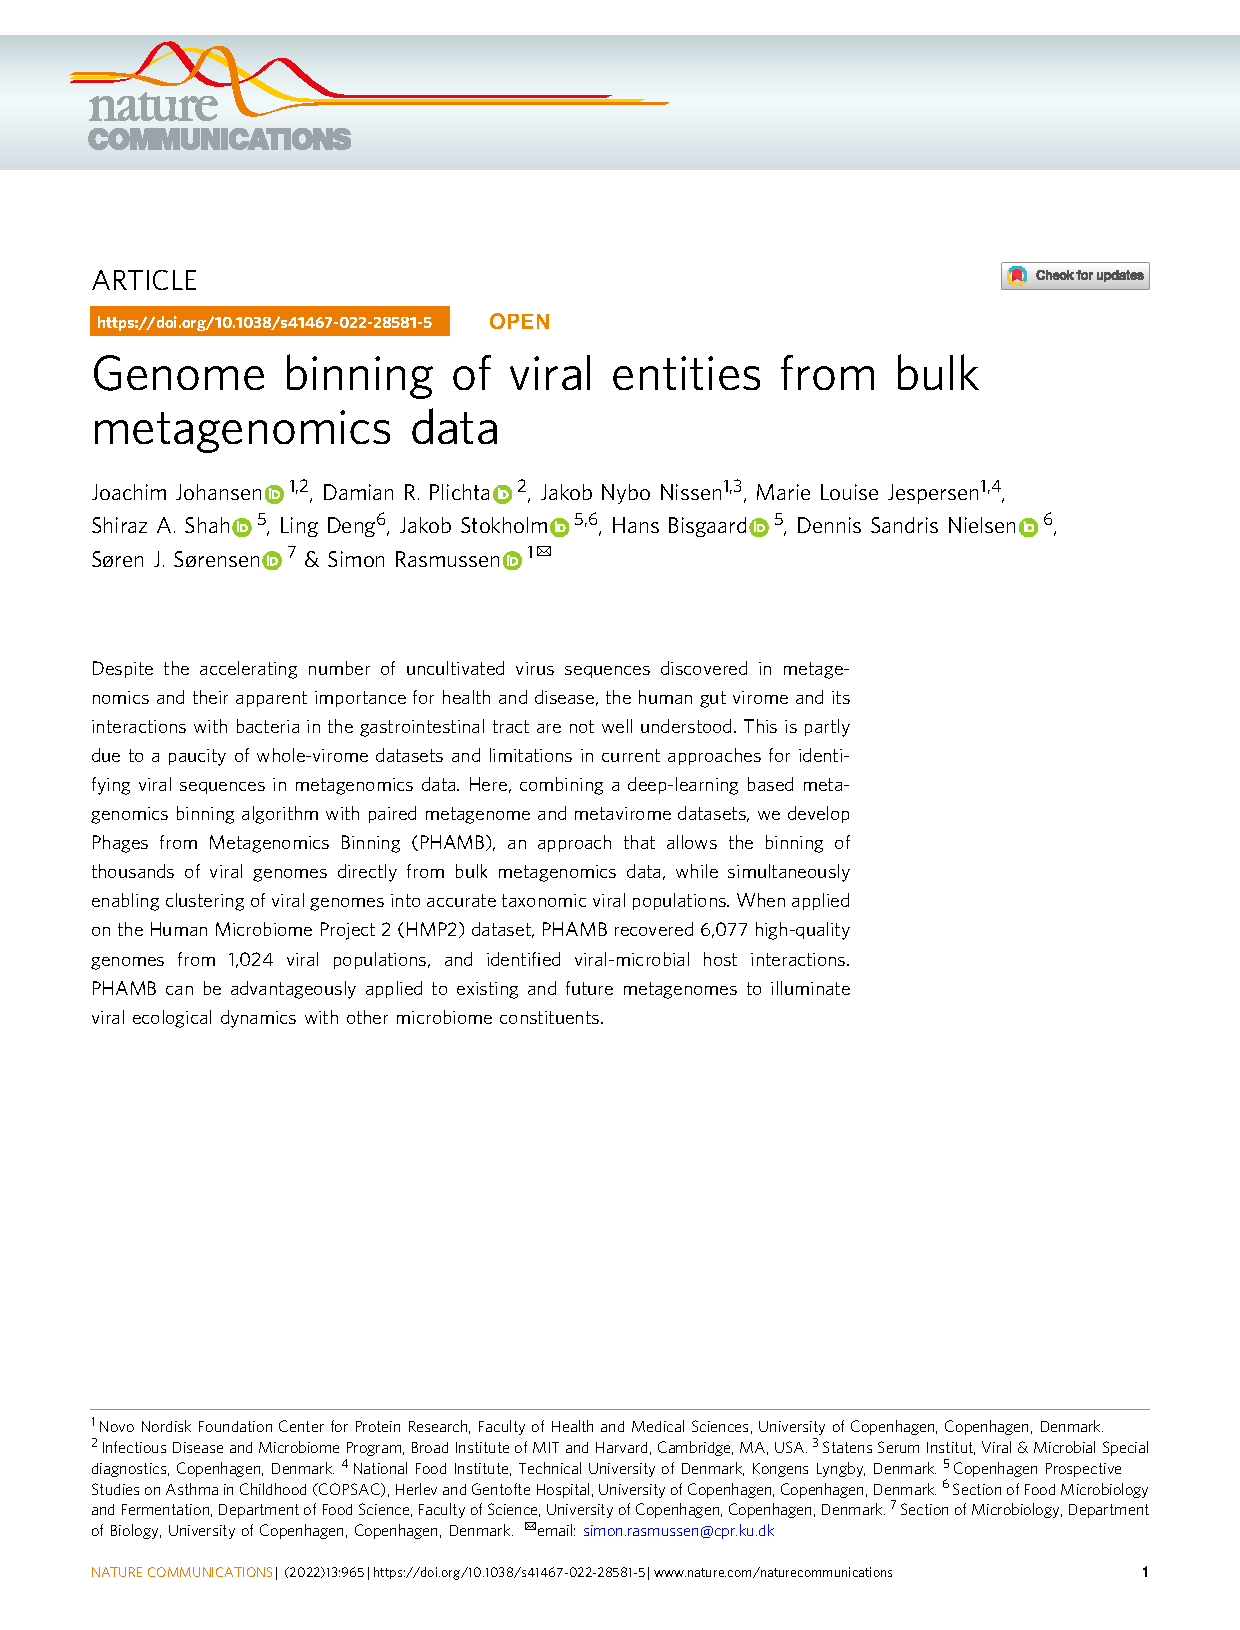
\includepdf[pages=-,scale=0.75,pagecommand=\thispagestyle{papers}]{papers/phamb.pdf}


\endgroup


%%%%% APPENDIX %%%%
\begingroup

\makepagestyle{papers}
\makeoddhead{papers}{\thepage}{}{\leftmark}
\makeevenhead{papers}{\leftmark}{}{\thepage}
\makeheadrule{papers}{\textwidth}{0.3pt}
\pagestyle{papers}
\aliaspagestyle{chapter}{papers}

\chapter{Appendix}

\section{Popular science article in Politiken}\label{appendix:politiken}

\includepdf[pages=-,scale=0.75,pagecommand=\thispagestyle{papers}]{appendix/politiken_phager.pdf}

\endgroup


% Giv kapitel nummer. 
\printbibliography[title={References}]


\end{document}